\section{Pianificazione}
La pianificazione di progetto viene suddivisa nelle seguenti fasi:
\begin{itemize}
    \item \textbf{Analisi};
    \item \textbf{Technology baseline e codifica del PoC$^{G}$};
    \item \textbf{Progettazione di dettaglio e codifica};
    \item \textbf{Verifica validazione e collaudo}
\end{itemize} 
Al momento viene presentata una pianificazione dettagliata delle prime 2 fasi. Ogni fase viene suddivisa in \textit{sprint}$^{G}$ secondo le regole
del framework \textit{SCRUM}$^{G}$ dalla durata di circa 1-2 settimane. 

\subsection{Analisi}
Nella fase di analisi il team \textit{Club Swendwich} si occupa di produrre i seguenti documenti: \textit{Analisi dei requisiti}, \textit{Piano di progetto}, \textit{Piano di Qalifica} e \textit{Glossario}.

\subsubsection{Backlog: Analisi}
{\renewcommand{\arraystretch}{1.5}
\begin{longtable}{p{0.27\linewidth}p{0.49\linewidth}p{0.15\linewidth}}
	\rowcolor[RGB]{33, 73, 50}
	\textcolor{white}{\textbf{Titolo attività}} & \textcolor{white}{\textbf{Descrizione}} & \textcolor{white}{\textbf{Data inizio}}\\
    
    \rowcolor[RGB]{216, 235, 171}
    Incremento \par \textit{Norme di Progetto} & Il gruppo prosegue con la stesura delle Norme di Progetto, concentrandosi sulle sezioni "Documentazione" e "Codifica". & 18-11-2021\\

    \rowcolor[RGB]{233, 245, 206}
    Verifica \par \textit{Norme di Progetto} & Il gruppo prosegue con la verifica del documento \textit{Norme di Progetto} & 18-11-2021\\
    
    \rowcolor[RGB]{216, 235, 171}
    Casi d'uso & Il gruppo esegue uno studio preliminare per individuare i casi d'uso principali. & 25-11-2021\\

    \rowcolor[RGB]{233, 245, 206}
    Requisiti & Il gruppo esegue uno studio preliminare per individuare i requisiti (funzionali, vincolo e prestazionali) principali. & 25-11-2021\\

    \rowcolor[RGB]{216, 235, 171}
    Incontro & Il gruppo fissa un incontro con il proponente per discutere dei casi d'uso individuati. & 30-11-2021\\ 
    
    \rowcolor[RGB]{233, 245, 206}
    \textit{Analisi dei requisiti} & Il gruppo redige il documento \textit{Analisi dei requisiti}. & 03-12-2021\\

    \rowcolor[RGB]{216, 235, 171}
    Verifica \par \textit{Analisi dei requisiti} & Il gruppo inizia la verifica del documento \textit{Analisi dei requisiti}. & 03-12-2021\\

    \rowcolor[RGB]{233, 245, 206}
    Analisi dei rischi & Il gruppo individua i rischi principali riscontrabili nello sviluppo del progetto. & 13-12-2021\\

    \rowcolor[RGB]{216, 235, 171}
    Modello di sviluppo & Il gruppo identifica il modello di sviluppo al quale fare riferimento. & 14-12-2021\\

    \rowcolor[RGB]{233, 245, 206}
    Pianificazione & Il gruppo identifica un metodo di pianificazione e individua le fasi principali e i relativi sprint$^G$ . & 14-12-2021\\

    \rowcolor[RGB]{216, 235, 171}
    \textit{Piano di Progetto} & Il gruppo inizia la stesura della documento \textit{Piano di progetto}. & 21-12-2021\\

    \rowcolor[RGB]{233, 245, 206}
    Verifica \par \textit{Piano di Progetto} & Il gruppo inizia la verifa del documento \par \textit{Piano di Progetto}. & 21-12-2021\\

    \rowcolor[RGB]{216, 235, 171}
    Preventivo & Il gruppo elabora i preventivi relativi alle fasi individuate e descritte nella sezione \par "\textit{Pianificazione}" del documento \textit{Piano di Progetto}. & 27-12-2021\\

    \rowcolor[RGB]{233, 245, 206}
    Consuntivo di periodo & Il gruppo elabora un consuntivo di periodo relativo al documento \textit{Piano di progetto}. & 27-12-2021\\

    \rowcolor[RGB]{216, 235, 171}
    Attuazione dei rischi & Il gruppo individua i rischi che si sono verificati nel corso del progetto & 30-12-2021\\

    \rowcolor[RGB]{233, 245, 206}
    \textit{Piano di Progetto} & Il gruppo prosegue con la stesura del documento \textit{Piano di progetto}. & 02-12-2022\\
    
    \rowcolor[RGB]{216, 235, 171}
    \textit{Glossario} & Il gruppo inizia a redigere il documento \textit{Glossario}. & 03-01-2021\\

    \rowcolor[RGB]{233, 245, 206}
    \textit{Piano di Qualifica} & Il gruppo inizia la stesura del documento \textit{Piano di Qualifica}. & 07-01-2022\\

    \rowcolor[RGB]{216, 235, 171}
    Verifica \par \textit{Piano di Qualifica,} \par \textit{Glossario} & Il gruppo inizia la verifica dei documenti \textit{Piano di Qualifica} e \textit{Glossario}. & 07-01-2022\\

    \rowcolor[RGB]{233, 245, 206}
    Verifica finale & Il gruppo inizia la verifica finale di tutti i documenti redatti & 31-01-2022\\

    \caption{Tabella riassuntiva del backlog relativo alla fase di analisi}
\end{longtable}
}

\subsubsection{Suddivisione in sprint$^G$ : Analisi}
\begin{itemize}
    \item \textbf{\textit{Sprint$^G$  1}: (dal 18-11-2021 al 03-12-2021)}\\
    Il gruppo si concentra sulle attività di: incremento delle \textit{Norme di Progetto} e relativa verifica, individuazione dei casi d'uso e dei requisiti.\\
    Il gruppo fissa una \textbf{milestone}$^G$  per il \textbf{03-12-2021} alla quale si aspetta di aver completato la parte relativa alla sezione "\textit{Casi d'uso}" e "\textit{Struttura requisiti}" nel documento \textit{Norme di progetto}.\\
    Il gruppo inoltre fissa il seguente incontro e redige i relativi verbali:
    \begin{itemize}
        \item Incontro con Zucchetti: 03-12-2021;
    \end{itemize}
    Il gruppo esegue la verifica dei verbali interni redatti in questo sprint.

    \item \textbf{\textit{Sprint$^G$  2}: (dal 03-12-2021 al 20-12-2021)}\\
    Il gruppo si concentra sulle attività di: stesura dell'\textit{Analisi dei requisiti} e relativa verifica, Individuazione dei rischi, scelta del modello di sviluppo e pianificazione delle fasi.\\
    Il gruppo fissa una \textbf{milestone}$^G$  per il \textbf{20-12-2021} alla quale si aspetta di aver completato per la maggior parte la stesura del documento \textit{Analisi dei requisiti}, e di essersi concordato sul contenuto delle prime sezioni relative al documento \textit{Piano di progetto}.\\
    Il gruppo inoltre redige e verifica i verbali relativi alle rinunioni verificatesi in questo sprint.

    \item \textbf{\textit{Sprint$^G$  3}: (dal 21-12-2021 al 06-01-2022)}\\
    Il gruppo si concentra sulle attività di: stesura del \textit{Piano di progetto} e relativa verifica, elaborazione di un preventivo e di un consuntivo di periodo, individuazione dei rischi e stesura del \textit{Glossario}.\\
    Il gruppo fissa una \textbf{milestone}$^G$  per il \textbf{01-01-2022} alla quale ci si aspetta di essersi concordati sul contenuto delle sezioni: "\textit{Preventivo}", "\textit{Consuntivo di periodo"} e "\textit{Attuazione dei rischi}".\\
    Il gruppo inoltre redige e verifica i verbali relativi alle rinunioni verificatesi in questo sprint.

    \item \textbf{\textit{Sprint$^G$  4}: (dal 07-01-2022 al 31-01-2022)}\\
    Il gruppo si concentra sulle seguenti attività: stesura del \textit{Piano di qualifica} e relativa verifica, verifica ed incremento del \textit{Glossario} e correzione generale dei documenti redatti.\\
    Il gruppo fissa una \textbf{milestone}$^G$  per il \textbf{31-01-2022} alla quale si aspetta di aver ultimato tutti i documenti necessari per la RTB e di averli verificati.\\
    Il gruppo inoltre redige e verifica i verbali relativi alle rinunioni verificatesi in questo sprint.

    \item \textbf{\textit{Sprint$^G$  5}: (dal 31-01-2022 al 07-02-2022)}\\
    Il gruppo si concentra sull'attività di verifica finale e di approvazione dei documenti redatti  e segnala le ore personali svolte per l'aggiornamento del "\textit{Consuntivo di periodo"}. \\
    Il gruppo fissa una \textbf{milestone}$^G$  per \textbf{07-02-2022} alla quale ci si aspetta di aver ultimato la verifica finale dei documenti e di averli approvati.\\
    Il gruppo inoltre redige e verifica i verbali relativi alle rinunioni verificatesi in questo sprint.
\end{itemize}
\newpage
\subsubsection{Diagramma di Gantt: Analisi}
\begin{figure}[h!]
    \centering
    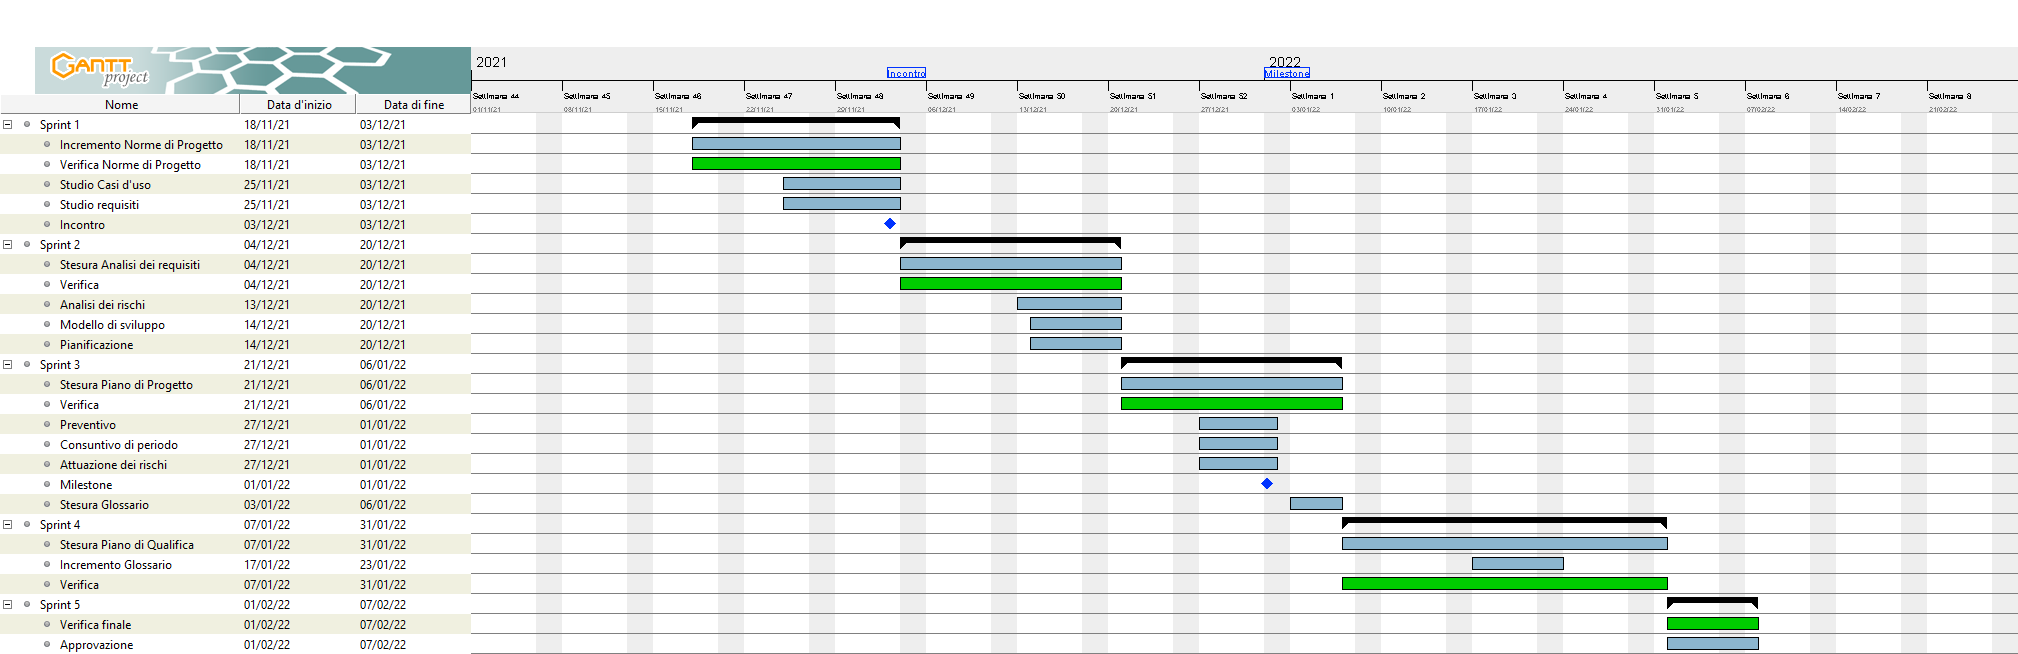
\includegraphics[scale=0.22]{../../assets/Diagrammi_Gantt/Analisi.png}
    \caption{Diagramma di Gantt - Analisi}
\end{figure}

\subsection{Technology baseline e codifica del PoC}
\subsubsection{Backlog: Analisi}
{\renewcommand{\arraystretch}{1.5}
\begin{longtable}{p{0.27\linewidth}p{0.49\linewidth}p{0.15\linewidth}}
	\rowcolor[RGB]{33, 73, 50}
	\textcolor{white}{\textbf{Titolo attività}} & \textcolor{white}{\textbf{Descrizione}} & \textcolor{white}{\textbf{Data inizio}}\\
    
    \rowcolor[RGB]{216, 235, 171}
    Individuazione \par delle tecnologie & Il gruppo si accorda sulle tecnologie migliori con le quali sviluppare il \textit{Proof of concept}. & 07-01-2022\\

    \rowcolor[RGB]{233, 245, 206}
    Funzionalità \par da sviluppare & Il gruppo concorda le funzionalità più importanti da sviluppare nel \textit{Proof of concept}. & 07-01-2022\\

    \rowcolor[RGB]{216, 235, 171}
    Incontro & Il gruppo fissa un incontro con il proponente per discutere delle scelte tecnologiche intraprese relativamente al \textit{Proof of concept}. & 10-01-2022\\

    \rowcolor[RGB]{233, 245, 206}
    Codifica \par \textit{caricamento dataset$^{G}$} & Il gruppo procede alla codifica della \par funzionalità di "\textit{caricamento del dataset$^{G}$}". & 15-01-2022\\

    \rowcolor[RGB]{216, 235, 171}
    Codifica \textit{Parsing}$^G$  & Il gruppo procede alla codifica della \par funzionalità di \textit{Parsing}$^G$ . & 17-01-2022\\

    \rowcolor[RGB]{233, 245, 206}
    Codifica \par \textit{Rendering$^G$ scatterplot$^{G}$} & Il gruppo procede alla codifica della \par funzionalità di \textit{Rendering$^G$  dello scatterplot$^G$ } & 20-01-2022\\

    \rowcolor[RGB]{216, 235, 171}
    Codifica \par \textit{Associazione assi} & Il gruppo procede alla codifica della \par funzionalità di \textit{associazione degli assi alle dimensioni$^{G}$}. & 22-12-2022\\

    \rowcolor[RGB]{233, 245, 206}
    Verifica e collaudo & Il gruppo procede alla verifica e al collaudo del \textit{Proof of concept}. & 31-01-2022\\

    \caption{Tabella riassuntiva del backlog relativo alla fase di Technology baseline}
\end{longtable}
}

\subsubsection{Suddivisione in sprint: Technology baseline e codifica del PoC}
\begin{itemize}
    \item \textbf{\textit{Sprint$^G$  1}: (dal 07-01-2022 al 15-01-2022)}\\
    Il gruppo si concentra sulle attività di: individuazione delle tecnologie da utilizzare e individuazione delle funzionalità da sviluppare.
    Il gruppo inoltre fissa i seguenti incontri:
    \begin{itemize}
        \item Incontro con Zucchetti: 10-01-2022;
    \end{itemize}
    Il gruppo in aggiunta redige e verifica i verbali relativi alle rinunioni verificatesi in questo sprint.

    \item \textbf{\textit{Sprint$^G$  2}: (dal 15-01-2022 al 31-01-2022)}\\
    Il gruppo si concentra sulle attività di codifica, in particolar modo vengono sviluppate le seguenti funzionalità: \textit{caricamento dataset$^{G}$}, \textit{Parsing}$^G$ , \textit{Rendering$^G$  Scatter Plot$^G$ } e \textit{Associazione degli assi alle dimensioni$^G$ }.\\
    Il gruppo fissa una \textbf{milestone}$^G$  per il \textbf{31-01-2022} alla quale si aspetta di aver codificato tutte le funzionalità necessarie al \textit{Proof of concept}.\\
    Il gruppo in aggiunta redige e verifica i verbali relativi alle riunioni verificatesi in questo sprint.

    \item \textbf{\textit{Sprint$^G$  3}: (dal 31-01-2022 al 07-02-2022)}\\
    Il gruppo si concentra sull'attività di verifica e collaudo del \textit{Proof of concept}.\\
    Il gruppo fissa una \textbf{milestone}$^G$  per il \textbf{07-02-2022} alla quale si aspetta di aver terminato tutte le attività di verifca e collaudo.\\
    Il gruppo in aggiunta redige e verifica i verbali relativi alle rinunioni verificatesi in questo sprint.
\end{itemize}

\subsubsection{Diagramma di Gantt: Technology baseline e codifica del PoC}
\begin{figure}[h!]
    \centering
    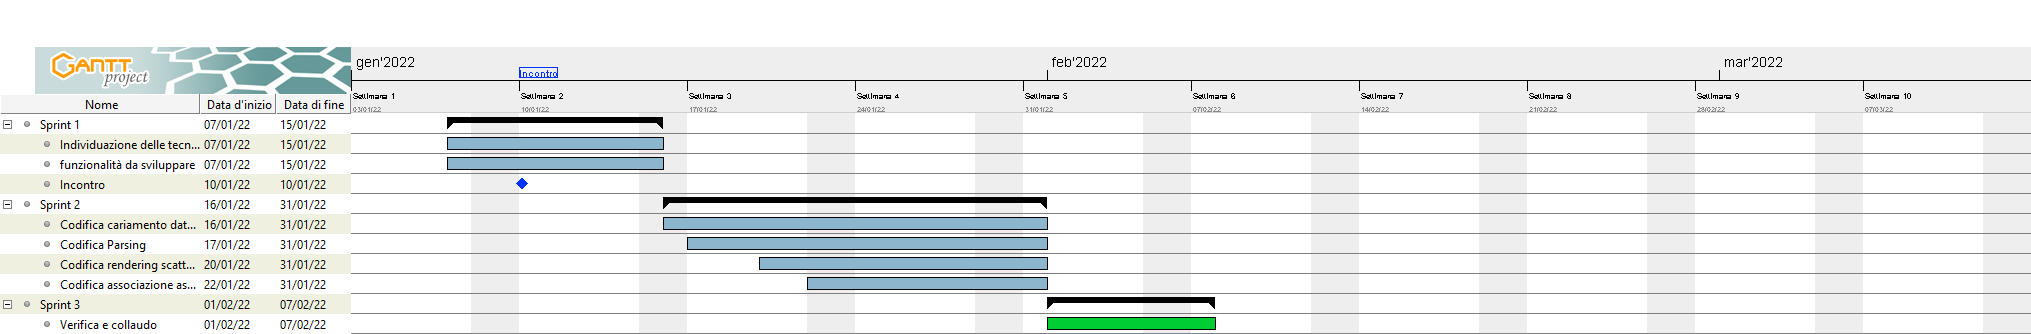
\includegraphics[scale=0.22]{../../assets/Diagrammi_Gantt/TB.png}
    \caption{Diagramma di Gantt - Technology baseline e codifica del PoC}
\end{figure}